\section{Анализ предметной области и разработка требований к проектируемому ПС}
\label{sec:analysis}

Тот факт, что работа над программным средством начинается с установления требований, сильно отражается на всем дальнейшем ходе работ. Если этот процесс выполнен недостаточно аккуратно, недостаточно точно, недостаточно адекватно, то от этого пострадают все остальные части процесса разработки.

Персонал, работающий с созданной системой, будет трактовать ошибки, искажения и неоднозначности как правильные требования, понапрасну тратя усилия не только на то, чтобы их внедрить, но и на то, чтобы затем от них избавиться.

Некоторые факты о важности требований приведены ниже:
\begin{itemize}
	\item 40 процентов бюджета тратятся на переделки;
	\item ошибки в требованиях являются наиболее частыми ошибками;
	\item стоимость ошибок в требованиях очень высока;
	\item за счет мультипликативного эффекта 70-80 процентов стоимости переделок тратится из-за ошибок в требованиях.
\end{itemize}

Перед формулированием требований необходимо изучить ряд вопросов, которые напрямую влияют на все дальнейшие этапы разработки. В частности, необходимо рассмотреть вопросы выбора платформ, архитектуры. По результатам анализа можно будет составить техническое задание к проектируемому программному средству, которое станет основой для составления функциональных требований.

\subsection{Сравнение нативных приложений и ботов} 
\label{sec:analysis:botsvsnative}

Чат-боты во многом привлекательны потому, что предоставляют возможность взаимодействовать с компьютерами в более естественной форме -- вместо работы с графическим интерфейсом достаточно сказать, какая задача требует выполнения. На данный момент чат-боты не развились до такого уровня, но определенный прогресс заметен уже сейчас. Например, для решения определенных задач уже сейчас пользователь может ввести определенную команду, а компьютер поймет и сделает то, что требуется.

Одно из безусловных препятствий к всеобщему проникновению ботов -- это синтаксис, который нужно помнить для взаимодействия с ними. В конце концов развитие технологий обработки языка и искусственного интеллекта позволит решить эту проблему -- компьютеру можно будет сказать почти что угодно, и он поймёт, о чём речь.

Хотя в большинстве существующих решений не содержится искусственного интеллекта, можно отметить, что ряд повседневных задач возможно решать путём переписки с автоматизированным агентом. Несмотря на то, что данные решения не отличаются сообразительностью и требуют знания определенного синтаксиса, возможность решать задачи посредством короткого обмена сообщениями делает этот процесс более легким и быстрым.

Простота разговорных интерфейсов может быть главным драйвером их распространения, но дискуссия о противостоянии ботов и приложений упускает кое-что из виду. Это контекст использования, и он, возможно, важнее чем простота. Большая доля привлекательности чат-ботов объясняется тем, что разговорные интерфейсы обладают уникальной возможностью интеграции в контекст, в котором находится пользователь. Чат-боты особенно востребованы в задачах, когда цена смены контекста слишком высока.

Возможность дать команду в чате -- это не только проще, чем сделать это через приложение. Она обеспечивает взаимодействие с минимумом отвлекающих факторов. По этой причине чат-ботам не обязательно нужно быть проще, чем аналогичные им приложения. Они должны соответствовать контексту, в котором пользователь решает определенную задачу.

Например, для того, чтобы узнать прогноз погоды, необязательно открывать приложение погоды на своем телефоне, достаточно спросить у ассистента и получить ответ, не отрываясь от текущего контекста.

Схожим образом боты в Slack позволяют делать всё что угодно в одной коллективной среде, что проще, нежели выполнение задач в разных интерфейсах и последующий сбор результатов в одно место. Интеграция вашего сервиса со Slack в виде бота снижает барьеры к принятию, потому что пользоваться сервисом можно будет в том же разговорном потоке, в котором уже ведутся дела.

Ставка на чат-ботов предполагает, что пользователи будут проводить всё больше времени в мессенджерах, и что пользоваться нужными сервисами при помощи ботов будет проще, чем открывать специальное приложение или сайт. В пользу такого развития событий уже говорит опыт Китая, в котором 650 млн человек проводят достаточно большой процент времени в мессенджере WeChat: они не просто общаются между собой, но и потребляют широкий ассортимент услуг.

Это причина, по которой Facebook возлагает большие надежды на бот-платформу для Messenger. Продукт, который позволит почти всем желающим поставлять контент или услуги через мессенджер. Компания идёт на этот шаг, рассчитывая на то, что в конечном итоге пользователи станут проводить большое количество свободного времени в Messenger — как в случае WeChat. Это манёвр, чтобы обойти iOS и Android как платформы для приложений, и сделать все сервисы доступными в Messenger.

Процесс адаптации может пойти медленно — пользователям потребуется время, чтобы привыкнуть к взаимодействию с ботами, но не трудно представить, что пользовательское поведение будет меняться по мере того, как элементов искусственного интеллекта в чат-платформах будет становиться больше, а грань между ботами и приложениями размоется.

Если боты победят, это произойдёт не по причине простоты использования, а из-за очевидной пользы от возможности встраивания в контекст, в котором пользователь уже решает свою задачу. Пользователи привыкнут разговаривать с ботами в силу удобства.

\subsection{Обзор существующих аналогов}
\label{sec:analysis:analogues}

Процесс управления категориями является ключевым в построении взаимодействия между пользователем и ботом. Для удобного и быстрого управление домашней бухгалтерией, требуется средство с интуитивно понятным интерфейсом.

В данном разделе представлены два самых популярных представителя ботов для контроля за персональными расходами: Greenz Bot и \linebreak WhereIsMyMoney Bot. Для каждого из аналогов будет даваться краткая характеристика, примеры работы, а также преимущества и недостатки данных программных продуктов.

\subsubsection{} Greenz Bot
\label{sec:analysis:analogues:greenz}

Бот обладает широким спектром функциональности, включая синхронизацию с Google таблицами, установку желаемой суммы, которую пользователь не хочет превышать в месяц. Использование бота предполагает написание пользователем категории и суммы, а также, если необходимо, указание даты и подкатегории. Принцип работы показан на рисунке \ref{fig:analysis:analogues:greenz}.

Возможность просмотра баланса отображена на рисунке \ref{fig:analysis:analogues:greenz_balance}.

Достоинства Greenz Bot:

\begin{itemize}
	\item Поддержка человеческого языка. Бот способен распознавать запросы пользователя, которые представляют собой предложения, сокращения и так далее. К примеру, командой <<бенз 150>>, пользователь добавит -150 единиц валюты в категорию Автомобиль.
	\item Возможность синхронизации с Google таблицами.
	\item Установка желаемой суммы, которую пользователь не хочет превышать за месяц.
\end{itemize}

Из минусов приложения можно выделить отсутствие следующих возможностей:

\begin{itemize}
	\item создание собственной категории;
	\item указание валюты.
\end{itemize}

\begin{figure}[!h]
	\centering
	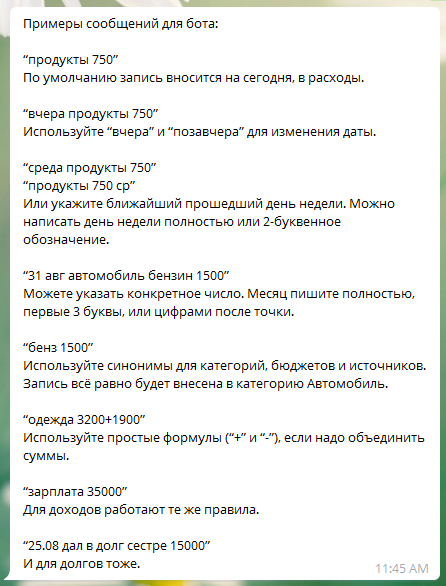
\includegraphics[scale=0.7]{greenzbot.png} 
	\caption{Принцип работы Greenz Bot}
	\label{fig:analysis:analogues:greenz}
\end{figure}

\newpage

\subsubsection{} WhereIsMyMoneyBot
\label{sec:analysis:analogues:whereismymoney}

Телеграм-бот WhereIsMyMoneyBot является хорошим помощником \linebreak для людей, желающих видеть, куда уходят их деньги. Бот поддерживает английский и русский языки, что помогает привлечь больше аудитории. Принцип работы бота описан на рисунке \ref{fig:analysis:analogues:whereismymoneybot}.

Приложение работает следующим образом: пользователь вводит сумму, которую потратил, а также категорию, состоящую из одного слова. Бот создает новую категорию и записывает в нее операцию.

Предлагается подробная история операций по категориям, а также, после каждого добавления операции предлагает статистику по количеству денег, потраченных на товары этой категории, всего потраченных денег в этом месяце, также сегодня. Помимо всего этого, можно настроить ежемесячные или еженедельные уведомления, что, безусловно, является большим преимуществом.

Достоинствами WhereIsMyMoneyBot являются:

\begin{itemize}
	\item возможность создания категорий;
	\item поддержка нескольких языков;
	\item наличие уведомлений.
\end{itemize}

\begin{figure}[!h]
	\centering
	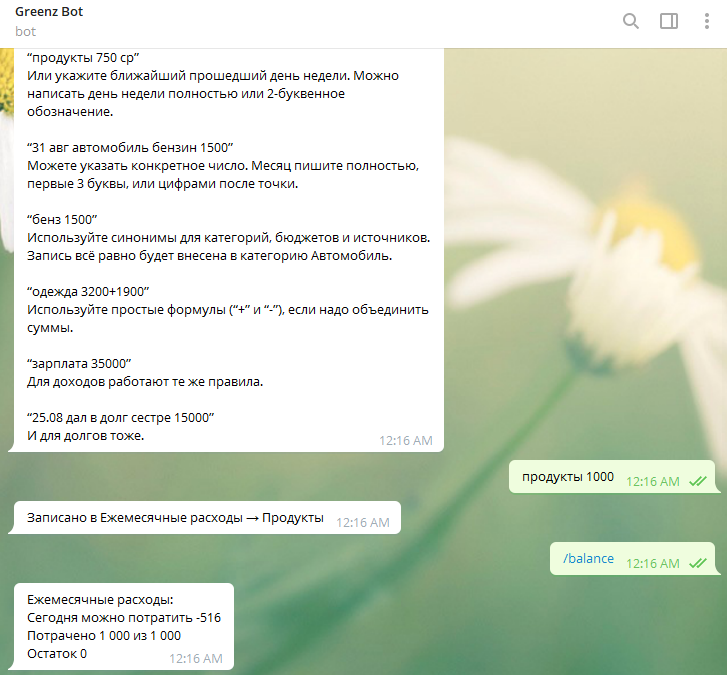
\includegraphics[scale=0.5]{greenzbot_balance.png} 
	\caption{Просмотр баланса в Greenz Bot}
	\label{fig:analysis:analogues:greenz_balance}
\end{figure}

\begin{figure}[!h]
	\centering
	
\includegraphics[scale=0.7]{whereismymoneybot.png} 
	\caption{Принцип работы WhereIsMyMoneyBot}
	\label{fig:analysis:analogues:whereismymoneybot}
\end{figure}

\newpage

Из минусов приложения можно выделить отсутствие следующих возможностей:

\begin{itemize}
	\item изменение категории;
	\item указание валюты.
\end{itemize}

После обзора аналогов был сделан вывод о том, что современные финансовые боты учитывают доходы, расходы, позволяют экспортировать статистику в различных форматах данных. Недостатками же является отсутствие возможности создания собственных категорий, а также отсутствие валюты.

В проектируемом программном средстве планируется использовать все достоинства существующих на рынке ботов, а также исправление их недостатков.




\subsection{Требования к проектируемому программному средству}
\label{sec:analysis:specification}

По результатам изучения предметной области, анализа литературных источников и обзора существующих систем-аналогов сформулируем требования к проектируемому программному средству.

\subsubsection{} Назначение проекта
\label{sec:analysis:specification:purpose}

Назначением проекта является разработка программного средства, автоматизирующего основные задачи участников учебного процесса университетов: управление расписанием, заданиями и коммуникацией.

\subsubsection{} Основные функции
\label{sec:analysis:specification:functions}

Программное средство должно поддерживать следующие основные фун\-к\-ции:

\begin{itemize}
	\item регистрация и аутентификация;
	\item поддержка системы ролей;
	\item отображение расписания занятий;
	\item отображение списка изучаемых дисциплин (для студентов) и преподаваемых дисциплин с типами занятий (для преподавателей);
	\item возможность управления индивидуальными заданиями и материалами по дисциплинам;
	\item отправка результатов выполнения индивидуальных заданий;
	\item оценивание/отклонение результатов выполнения заданий;
	\item управление очередями на защиту индивидуальных заданий;
	\item отправка сообщений другим пользователям системы;
	\item управление списками групп, их отображение со всеми выставленными оценками;
	\item возможность проверки посещения занятий.
\end{itemize}

\subsubsection{} Требования к входным данным
\label{sec:analysis:specification:inputs}

Входные данные для программного средства должны быть представлены в виде вводимого пользователем с помощью клавиатуры текста и выбора доступных опций пользовательского интерфейса.

Должны быть реализованы проверки вводимых данных на корректность с отображением информации об ошибках в случае их некорректности.

\subsubsection{} Требования к выходным данным
\label{sec:analysis:specification:outputs}

Выходные данные программного средства должны быть представлены посредством отображения информации с помощью различных элементов пользовательского интерфейса.

\subsubsection{} Требования к временным характеристикам
\label{sec:analysis:specification:timing}

Производительность программно-аппаратного комплекса должна обеспечивать следующие временные характеристики: время реакции не запрос пользователя не должно превышать 1 секунды при минимальной скорости соединения 1 МБит/с. Допускается невыполнение данного требования в случае, когда невозможность обеспечить заявленную производительность обусловлена объективными внешними причинами.

\subsubsection{} Требования к надежности
\label{sec:analysis:specification:reliability}

Надежное функционирование программы должно быть обеспечено выполнением следующих организационно-технических мероприятий:

\begin{itemize}
	\item организация бесперебойного питания;
	\item выполнение рекомендаций Министерства труда и социальной защиты РБ, изложенных в Постановлении от 23 марта 2011 г. «Об утверждении Норм времени на работы по обслуживанию персональных электронно-вычислитель\-ных машин, организационной техники и офисного оборудования»;
	\item выполнение требований ГОСТ 31078-2002 <<Защита информации. Испытания программных средств на наличие компьютерных вирусов>>;
	\item необходимым уровнем квалификации пользователей.
\end{itemize}

Время восстановления после отказа, вызванного сбоем электропитания технических средств (иными внешними факторами), нефатальным сбоем операционной системы, не должно превышать времени, необходимого на перезагрузку операционной системы и запуск программы, при условии соблюдения условий эксплуатации технических и программных средств. Время восстановления после отказа, вызванного неисправностью технических средств, фатальным сбоем операционной системы, не должно превышать времени, требуемого на устранение неисправностей технических средств и переустановки программных средств.

Отказы программы возможны вследствие некорректных действий пользователя при взаимодействии с операционной системой. Во избежание возникновения отказов программы по указанной выше причине следует обеспечить работу конечного пользователя без предоставления ему административных привилегий.

\subsubsection{} Требования к аппаратному обеспечению серверной части
\label{sec:analysis:specification:server_requirments}

ЭВМ, на которой должна функционировать серверная часть программного средства, должна обладать следующими минимальными характеристиками:

\begin{itemize}
	\item процессор Intel Core i5 с тактовой частотой 2 ГГц;
	\item жесткий диск объемом 100 Гб;
	\item оперативная память 4 Гб;
	\item сетевая карта Ethernet 100 МБит/с.
\end{itemize}

Также для функционирования серверной части требуется установленный Apache HTTP Server, который является кроссплатформенным программные средством, вследствие чего вопрос о целевой операционной системе не рассматривается. Кроме того, процедуры установки и настройки данного веб-сервера выходят за рамки данного проекта и также не рассматриваются.

\subsubsection{} Требования к аппаратному обеспечению клиентской части
\label{sec:analysis:specification:client_requirments}

Клиентская часть программного средства должна функционировать на ЭВМ со следующими минимальными характеристиками:

\begin{itemize}
	\item процессор Intel Pentium 4 с тактовой частотой 2 ГГц и более;
	\item оперативная память 2 Гб и более;
	\item сетевая карта Ethernet 10/100 Мбит.
\end{itemize}

Для корректной работы программного средства необходим один из следующих браузеров с соответствующей минимальной версией:

\begin{itemize}
	\item Google Chrome 49;
	\item Vivaldi 1.0;
	\item Opera 34;
	\item Mozilla Firefox 43;
	\item Apple Safari 9.0;
	\item Microsoft Edge 20.
\end{itemize}

\subsubsection{} Выбор технологий программирования
\label{sec:analysis:specification:language}

Язык программирования, на котором будет реализована система, заслуживает большого внимания, так как вы будете погружены в него с начала конструирования программы до самого конца. Исследования показали, что выбор языка программирования несколькими способами влияет на производительность труда программистов и качество создаваемого ими кода. Если язык хорошо знаком программистам, они работают более производительно. Данные, полученные при помощи модели оценки Cocomo II, показывают, что программисты, использующие язык, с которым они работали три года или более, примерно на 30\% более продуктивны, чем программисты, обладающие аналогичным опытом, но для которых язык является новым~\cite{software_cost_estimation}. В более раннем исследовании, проведенном в IBM, было обнаружено, что программисты, обладающие богатым опытом использования языка программирования, были более чем втрое производительнее программистов, имеющих минимальный опыт~\cite{method_of_programming_measurement_and_estimation}.

Язык программирования \typescript, указанный в задании на дипломное проектирование, является кроссплатформенным языком программирования. Данный ЯП представляет собой надмножество языка JavaScript, что означает, что их объединяют общие синтаксис и семантика управляющих конструкций; ключевой отличительной особенностью является возможность использования строгой типизации, что значительно упрощает статические проверки кода. Кроме того, он компилируется в обычный JavaScript, что означает возможность запуска кода в любом браузере или движке, который поддерживает стандарт ECMAScript 3 или более новый \cite{typescript}. 

Несмотря на то, что \typescript, так же как и JavaScript, изначально предназначался для запуска в браузере клиента, в настоящее время разработаны фреймворки, позволяющие использовать его для разработки под различными платформами: Windows 10 \cite{modern_apps}, iOS, Android \cite{nativescript} и другие.

Исходя из достоинств данного языка программирования, можно сделать вывод, что он наиболее подходящий для решения проблем, схожих с поднимаемыми в данной пояснительной записке. Именно поэтому \typescript и выбран как основной язык программирования в задании к текущему дипломному проекту.

Однако, выбранный язык программирования является средством для программирования клиентской части приложения. Поскольку для приложения в любом случае понадобится база данных, то есть два варианта: 

\begin{itemize}
	\item осуществлять запросы к БД напрямую с клиентского приложения;
	\item реализовать серверную прослойку между клиентской частью и базой данных.
\end{itemize}

Первый подход крайне небезопасен: очень опасно предоставлять открытый доступ к БД. В это же время, второй способ, помимо ее сокрытия, предоставляет возможность проверки подлинности и предоставления прав пользователям. В связи с этим появляется проблема выбора технологий для серверной части. Основным влияющим фактором является имеющийся опыт команды разработки, в связи с чем была выбрана технология .Net и язык программирования \csharp. 

.NET Framework — программная платформа, выпущенная компанией Mi\-c\-ro\-soft в 2002 году. Она была призвана решить ряд наболевших проблем в мире разработки ПО, скопившихся на момент ее выхода, что отражено в целях, которые
были поставлены в ходе ее разработке. 

При разработке платформы .NET учитывались следующие цели~\cite{msdn_dotnet}:

\begin{itemize}
	\item Обеспечение согласованной объектно-ориентированной среды про\-г\-ра\-мми\-ро\-ва\-ния для локального сохранения и выполнения объектного кода, для локального выполнения кода, распределенного в Интернете, либо для удаленного выполнения.
	\item Обеспечение среды выполнения кода, минимизирующей конфликты при развертывании программного обеспечения и управлении версиями.
	\item Обеспечение среды выполнения кода, гарантирующей безопасное выполнение кода, включая код, созданный неизвестным или не полностью доверенным сторонним изготовителем.
	\item Обеспечение среды выполнения кода, исключающей проблемы с производительностью сред выполнения сценариев или интерпретируемого кода.
	\item Обеспечение единых принципов работы разработчиков для разных типов приложений, таких как приложения Windows и веб-приложения.
	\item Разработка взаимодействия на основе промышленных стандартов, которое обеспечит интеграцию кода платформы .NET Framework с любым другим кодом.
\end{itemize}

Несмотря на то, что платформа .Net поддерживает несколько языков программирования, основным является язык \csharp. Он является простым, современным, объектно-ориентированным, обеспечивающим безопасность типов языком программирования. Он соответствует международному стандарту Европейской ассоциации производителей компьютеров — стандарт ECMA-334, а также стандарту Международной организации по стандартизации (In\-ter\-na\-ti\-o\-nal Standards Organization, ISO) и Международной электротехнической комиссии — стандарт ISO/IEC 23270. Компилятор Microsoft \csharp для .NET Framework согласуется с обоими этими стандартами~\cite{msdn_charp}.

Одной из сред программирования, которая поддерживает одновременно и \csharp, и \typescript, является Microsoft Visual Studio, которая входит в линейку продуктов компании Microsoft, включающих интегрированную среду разработки программного обеспечения и ряд других инструментальных средств. Она включает в себя редактор исходного кода с поддержкой технологии In\-tel\-li\-Sen\-se и возможностью рефакторинга кода. Встроенный отладчик может работать как отладчик уровня исходного кода, так и как отладчик машинного уровня. Visual Studio позволяет создавать и подключать сторонние дополнения для расширения функциональности практически на каждом уровне, включая добавление поддержки систем контроля версий исходного кода, добавление новых наборов инструментов или инструментов для прочих аспектов процесса разработки программного обеспечения. Именно поэтому она и выбрана в качестве основной среды программирования.

Язык программирования \typescript~можно использовать для создания приложений для различных платформ. Для проектируемого программного сре\-д\-с\-т\-ва актуальны следующие характеристики:
\begin{itemize}
  \item нет необходимости в организации ресурсоемких вычислений;
  \item желательна возможность использования мгновенных уведомлений и оповещений;
  \item желательна доступность приложения на различных устройствах.
\end{itemize}

По результатам обзора возможных платформ, представленных в пункте~\ref{sec:analysis:literature:platforms}, было принято решение выбрать основной для разработки платформу веб-приложений. После завершения разработки первой версии программного средства будет рассматриваться вопрос разработки мобильного приложения.

Фактор опыта использования оказал влияние на выбор системы управления базами данных для разрабатываемого приложения. СУБД \nezaboodka является особенно приспособленной для веб-приложений. Ее отличительной особенностью является возможность масштабируемости, а также отказоустойчивость. Основным способом взаимодействия с данной СУБД является предложенная разработчиком клиентская библиотека на языке \csharp.

Сформулированные требования позволят осуществить успешное проектирование и разработку программного средства.
